\graphicspath{{chapters/images/09/}}

\chapter{Staphylococcus aureus}

\emph{Staphylococcus aureus} is a gram positive bacterim (it has a peptidoglican layer into the cell wall) and it is a facultative anaerobe bacterium. This is very crucial for \emph{S. aureus} epidemiology because it is able to colonize nostrils where there is oxygen, but it is also able to colonize organs that are inside the body. It is  one of the main players in common food poisoning. It is also involved in the menstrual toxic shock syndrome. It plays a key role, also, in other serious disease, like osteomyelitis which in an infection of the bones or sepsis that is a systemic infections. 
It is a common skin colonizer and for this reason 25$\%$ of the people probably have \emph{S. aureus} in their body, but it is also the cause of very bad skin infection. 
The main reason for \emph{S. aureus} to be tricky to treat because of is immune evasion strategies.

\section{Immune evasion strategies}

\emph{S. aureus} has two different main strategies that used in order to stop the immune system of the host from getting rid of it. 

\begin{enumerate}
    \item It prevents the engagement of the host immune system, so it is not be recognized by the host immune system. That is done by different proteins that are present on the  surface of \emph{S. aureus}.
    \begin{itemize}
        \item Adhesins bind complement factors to inhibit complement activation cascade.
        \item Leukocidins are instead a number of toxins that are selectively killing the adapting immune cells, so killing those immune cells that would be able to kill \emph{S. aureus}. 
        \item Immunoglobulin binding proteins bind and immobilize IgGs, so they cannot start the cascade of activation of the immune systems.
        \item Proteases that cleave the immunoglobulin that are responsible for the activation.
    \end{itemize}
    There are four different kind of classes of proteins that are all try to hide the \emph{S. aureus} to the host immune system. 
    \item Overactiovation of the non-specific immune system. It is able to trigger a lot of inflammation to cytokine release, that is a non-specific reaction of the body, and also to facilitate invasion of the so-called non-professional phagocytes, the neutrophiles. There is the production of autholysins, that facilitate invasion of non-professional phagocytes, and super-antigens, that activate T cells and trigger the cytokine release. This could be an advantage to \emph{S. aureus} because when a neutrophiles phagocytes a bacterium or any pathogen can happen that the microbiome is uptaken by the neutrophile, is killed through degranulation and ROS production. The neutrophile then undergoes apoptosis and it is removed by macrophages and so we have a resolution of the infection. 
    If \emph{S. aureus} is present, we have the neutrophile that uptake him. However, \emph{S. aureus} stops the apoptosis of the neutrophile and is able to divide inside it and be screened by the immune system of the host and then, with the leukocidins, it can cause some holes in the neutrophile and also the release of its content outside causing an extra inflammation. 
\end{enumerate}

\section{Antibiotic resistance in \emph{S. aureus}}

In the $1940$s we have the introduction of penicillin G that is quickly followed by emergence of resistance, the penicillinase. 
In $1959$ was found the methicillin, a semisynthetic penicillinase-resistant $\beta$-lactam antibiotics, but in $1960$ we have already some cases of resistance to this antibiotic from an hospital in UK (MRSA). In $1960$ MRSA emerged in many countries. 

\subsection{Methicillin-resistant \emph{S. aureus} (MRSA)}

\emph{S. aureus} is resistant to \emph{beta}-lactam and is also able to acquire other resistances, event to last resource antibiotics, like vancomycin, linezolid, daptomycin.

Because \emph{S. aureus} is a gram-positive bacterium, the peptidoglycan layer of the cell wall is extremely important for the correct assembly of the cell membrane and the $\beta$-lactam antibiotics have the ability to act as substrate analog causing an impaired transpeptidation of the peptidoglycan and the creation of a defective cell wall during cell division.

\begin{enumerate}
    \item In absence of $\beta$-lactam antibiotics, we have the normal cell-wall biosynthesis.
    \item In presence of $\beta$-lactam antibiotics, we have the binding of the antibiotic to the PBP active site and therefore the peptidoglycan cannot be transpeptidated and the peptidoglycan layer of the cell wall cannot be produced and so we have the cell death during division. 
    \item In presence of the $\beta$-lactam antibiotics, but with mutated PBP (PBP$2$a, aka MecA), $\beta$-lactam is not able to bind the modified PBP. So, the peptidoglycan can be normally transpeptidated and \emph{S. aureus} can produce the cell wall and proliferate. 
\end{enumerate}

\subsection{Methicillin resistance: where is it encoded?}

The resistance to methicillin, but more in general to $\beta$-lactam, is not encoded on a plasmid. It is encoded on a mobile genetic element that is called staphylococcal chromosome cassette \emph{mec} (SCC\emph{mec}). SCC\emph{mec} are mobile genetic elements that are wide spread across staphylococci genome. They commonly carries genes that might confers some increased fitness for specific environments. This type of mobile genetic elements can be easily integrated into the genome and also can easily excises from the genome. That means that is really easy for a MSSA to integrate the mobile genetic element in case of a strong selective pressure that might be given by the presence of antibiotic. When the antibiotic is not more present, it is easy for MSSA to excise the mobile genetic element and return to the basic state of methicillin asset of the \emph{S. aureus}. 
The mobile genetic element is not maintained inside the cell. It is integrated into the cell or it is excised and released outside.

\subsection{Methicillin-resistant \emph{S. aureus} (MRSA)}
S. aureus is not well recognized for the problems that it causes. There are 80 thousands new patients per year in US that have invasive infections (not colonization), so that means that are people that are sick. The mortality rate is $20\%$. 
    Hospitalize patients, immune compromise patients or patients with conditions like cystic fibrosis are very expose to \emph{S. aureus}. This is why, in 2017, the World Health Organization insert \emph{S. aureus} resistant to meticillin and partially resistant to vancomycin or completely as a high priority bug for the research and the development of new antibiotics. Is the fifth one in the list.
An article of three years ago estimated about 5 millions deaths associated with bacterial antibiotic resistances (not \emph{S. aureus} only) in $2019$. The World Health Organization has estimated that by 2025 there will be 10 millions deaths per years because of antibiotic resistance. 

\subsubsection{\emph{S.aureus} worldwide}
There are lot of studies that focused on MRSA or \emph{S. aureus} infections, but the problem is that there are quite biases toward specifically lineages. With the term lineages, we refer to a specific strain or a group of strains that are known to be particularly hyper-virulent or resistant or affecting a specific population (e.g. cystic fibrosis patients). So, only a part of the pool of infections that \emph{S. aureus} can cause. There is a greater underestimation of the strains that are sensitive to methicillin for no reason because if \emph{S. aureus} can be sensitive to methicillin, so it can be resistant to all the other antibiotics. 
There is a great variability in MRSA that can change epidemiology:
\begin{itemize}
    \item $60$s-$70$s. There were lots of hospitals associated infections, so people go to the hospital, get a surgery and get \emph{S. aureus}. Also, nowadays \emph{S. aureus} is a key player in post-surgery infections. 
    \item $80$s-$90$s. The community start talking about community-associated \emph{S. aureus} infections and methicillin resistance of \emph{S. aureus} because the study starting focusing on the dissemination, also in healthy people.
    \item $2000$s. There was a great studies on livestock-associated MRSA. Zoonotic infections are pretty relevant, but treatment with antibiotics cause resistances in that community. Livestock diseases and resistances are serious consequences.  
\end{itemize}

\section{Whole genome epidemiology, characterization, and phylogenetic reconstruction of \emph{S. aureus} strains in a pediatric hospitals}

This work is a full pipeline of what you do if you want to do a survey of the general populations of \emph{S. aureus} in a specific place. 

\begin{figure}[h]
\centering
\caption{}
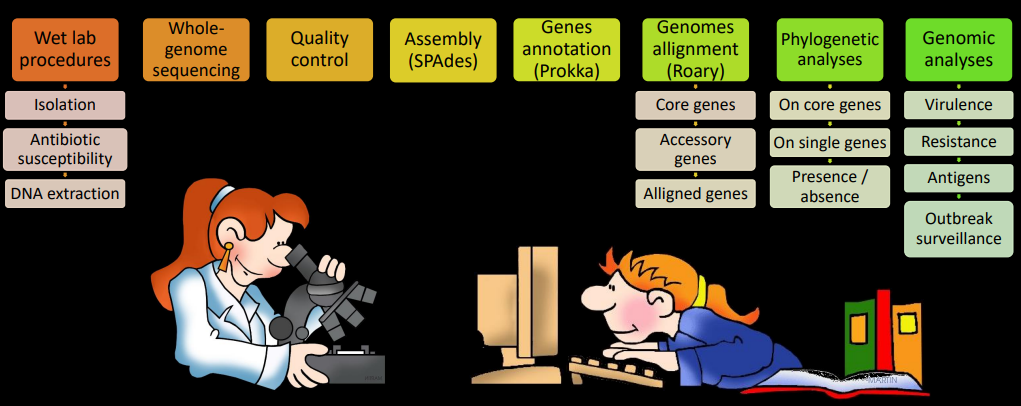
\includegraphics[width=1.0\textwidth]{Workflow.png}
\caption{Wet and dry lab workflow}
\end{figure}

\subsection{Methods}

They had $11$ operative units that were quite separated. 

They started with $234$ \emph{S. aureus} isolates:

\begin{itemize}
    \item antibiotic susceptibility test in vitro
    \item whole-genome sequencing
\end{itemize}

After, they selected 184 (N50>50k) so they discarded 50 of the isolates because they want high-quality genome to do a number of analysis.
They did not select patients on the base of their infections or the status, because some of these people were not there because of \emph{S. aureus}.
People come from different departments such as cystic fibrosis , day hospital, first aid,  immunology, infections diseases, intensive care, oncology, pediatrics, respiratory physio-pathology, surgery or week hospital. 
135 single patients were selected because them wanted all single patients isolates. 

\begin{itemize}
    \item Average nr of contigs = $51$ ($12$-$138$)
    \item Average N$50$ = $206$k ($50$k-$970$k)
\end{itemize}

Also the materials of the samples were different. They had some bronchoaspiration material, sputum, nasal swab, pharyngeal swab, lesion swab and other materials, which included blood and similar.


\subsection{Typing methods}

Usually the typing of \emph{S. aureus} is based on four different typing methods. All these methods have been created for wet-lab work. They are:

\begin{enumerate}
    \item Multilocus sequence typing (MLST).
    \item \emph{S. aureus} proteins A (spa). It is one of the major determinant of virulence on \emph{S. aureus}.
    \item Staphylococcal cassette chromosome \emph{mec} (SSC\emph{mec}). Looked at the presence or absence.
    \item Proton-Valentine Leukocydin (PVL). Looked at the presence or absence.
\end{enumerate}

\subsection{MLST}

\begin{enumerate}
    \item Characterizing isolates by sequencing fragments of house-keeping genes. 
    \item Each isolate is characterized by its allelic profile at the house keeping loci $\xrightarrow[]{}$ sequence type (ST). 
    \item Based on multilocus enzyme electrophoresis (MLEE). We should do that for all the genes and because the large amount of PCRs ($945$) it is not really fast. The allelic profile is much faster since you need only to sequence and then compare. 
\end{enumerate}

MLST take fragments of house-keeping genes and look at the sequence of them to assign an allelic profile. That means that if we have $3$ strains A, B and C, if we look at the first gene (abcZ) and at a some position we have G it will be allele of type $1$, while if we have a C it will be of type $2$. We do this kind of analysis with all the genes. Then we put the allelic profiles of all the $7$ house-keeping genes that are important for \emph{S. aureus} and we have a sequence of numbers that we can compare to a database of sequence types to know of lineage we are looking at. 

\subsection{Spa-typing}

\begin{enumerate}
    \item Single locus DNA-sequencing of the repeat region of the Staphylococcus protein gene (spa).
    \item Can be used to further discriminate STs. 
    \item Repeats are assigned a numerical code and the spa-type is deduced from the order of repeats. 
\end{enumerate}

The Staphylococcus protein A typing looks at the differences in the repeat sequence that is internal in the Staphylococcus protein A gene. This gene has a part of repeats that can be in different positions. The order of the repeats is the determinant of the spa-type. 
They have done 135 PCRs.

\subsection{SCC\emph{mec}}

During the sequencing of the region containing \emph{mecA} it was find a distinct mobile genetic element named the staphylococcal chromosome cassette \emph{mec} (SCC\emph{mec}).

\begin{figure}[h]
\centering
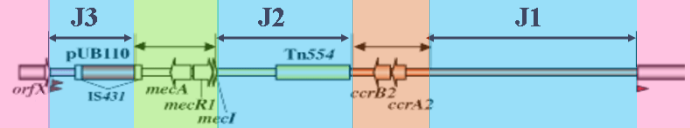
\includegraphics[width=0.6\textwidth]{SCCmec.png}
\caption{}
\end{figure}

\begin{enumerate}
    \item \emph{mec} gene complex (\emph{mecA} + \emph{mecI} and \emph{mecR}). \emph{mecA} is responsible for the resistance, \emph{mecI} is the inhibitor of \emph{mecA}, \emph{mecR} ($1$ or $2$) is the inhibitor of the inhibitor (\emph{mecI}). \emph{mecA} is always present, the other two might be present or not and that will give a typing of the cassette.
    \item Cassette chromosome recombinase (\emph{ccr}) gene complex helps making the typing of the cassette. 
    \item $3$ Joining (J) regions are responsible for other resistances. And can be also used for subtyping regions. 
    \item Specific inverted and directed repeats containing the insertion site recognized by the \emph{ccr}-encoded recombinase. 
    \item $11$ (from I to XI) types of cassette, different in size and gene content
    \begin{itemize}
        \item SCC\emph{mec} typing on \emph{mec} and \emph{ccr} gene complexes
        \item Suptyping on J regions
    \end{itemize}
\end{enumerate}

There were made $675$ PCRs.

\subsection{PVL}

PVL is a regarded as an important indicator of \emph{S. aureus} virulence. The PVL factor is encoded in a prophage that secretes two toxins LukS-PV and LukF-PV. It is a good indicator of how invasive an infections can be.

\begin{itemize}
    \item assemble in the membrane of host white blood cells, monocytes, and macrophages. 
    \item form a ring with a central pore through which immune-cell contents leak
    \item the ring also acts as a superantigen and we have the suppression of adaptive immune response. 
\end{itemize}

There were made $135$ PCRs.
In total were made $1890$ PCRs to get the typing of the community. 

\subsection{The cohort}

There are $1464$ core genes that are present in at least 99$\%$ of the strains and there are some trees that are quite specific and they matched very well with the MLST typing. We have lot of information about the sample type, the operative unit, the PVL presence, the SCC\emph{mec} type and also the presence of virulence genes. For virulence genes they made a list of all the very well known genes that are thought to be virulence genes in \textit{S. aureus} and they just reported the presence or absence of them. In this little cohort there were:

\begin{itemize}
    \item $28$ STs ($14$ CCs)
    \item $41$ \emph{spa}-types
    \item $4$ SCC\emph{mec} types 
    \item $27.4\%$ PVL+
\end{itemize}

There are $8373$ core genes in total that are present in at least 1 isolates.
  
\subsection{Typing highlights common clones and newly sequenced ones}

\subsection{Co-presence of local, global, animal-associated and hypervirulent clones}

\begin{figure}[h]
\centering
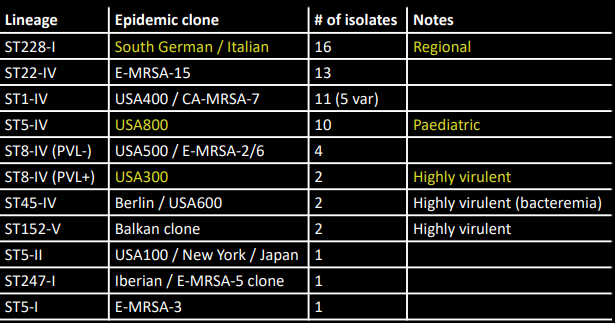
\includegraphics[width=0.6\textwidth]{Highlights.png}
\caption{}
\end{figure}

\begin{enumerate}
    \item Highly virulent STs
    \begin{itemize}
        \item USA$300$ ST$8$-SCC\emph{mec}IV PVL+
        \item ST$239$ HA-MRSA $\xrightarrow[]{}$ high transmissibility and quickly develops into bacteria
        \item ST$45$-SCC\emph{mec}IV $\xrightarrow[]{}$ bacteremia, MSSA isolated from infectious diseases
        \item ST$121$ MSSA $\xrightarrow[]{}$ from lesion swabs
        \item ST$152$-SCC\emph{mec}V $\xrightarrow[]{}$ severe infections
    \end{itemize}
    \item Livestock-associated MRSA (LA-MRSA), like ST398 and ST97. Increasing in non at-risk individuals 
    \item They found also ST$395$ lineage that is very peculiar and it is usually not found in humans. It was find in a child that was not at risk. It is particularly interesting because he can exchange DNA with the coagulase negative \emph{S. aureus} (CoNS) because it has modified wall teichoic (WTA).
\end{enumerate}
Livestock-associated MRSA (LA-MRSA) cause mastitis. They found also in children that were not expose. 

\subsection{Genomic signature of chronic versus acute \emph{S. aureus} infections}

Correlation of specific departments with virulent STs and PVL+:

\begin{itemize}
    \item CF + intensive care $\xrightarrow[]{}$ PVL + ST$121$ 
    \item first aid + infectious diseases $\xrightarrow[]{}$ PVL
    \item infectious diseases $\xrightarrow[]{}$ ST$45$
\end{itemize}

Sample types: 

\begin{itemize}
    \item lesion swabs $\xrightarrow[]{}$ MSSA, ST$121$ and PVL. Here they found virulent and not resistant infections, and that make sense because it is an acute infections.
    \item Lung isolates (bronchoaspiration material + sputum) $\xrightarrow[]{}$ ST$128$, PVL and MSSA. 
\end{itemize}

They observed that chronic infections are usually less virulent, while normally acute infections are more virulent. 

\subsection{Variability in SCC\emph{mec} cassettes}

They took cassettes and they did genomically analysis to specifically check the genes that are present. When you focused on a specific part of the genome, you can look in depth which genes are present or absent and also the functions of each genes. They found two cassettes harboring extra genes that were resistant at antibiotics (kanamycin, bleomycin and trimethoprim). 

\subsection{Diversity of virulence factors and antigens}

You can look also at specific class of genes, like immune evasion genes. Some immune invasion genes are present in almost all of the isolates. The resistant to vancomycin is never present. But is present the resistant to penicillin. 
There is only one sample (first aid) positive for Edin (epidermal cell differentiation inhibitor) → translocation into the bloodstream.
One USA300 isolate positive for the arginine catabolic mobile element (ACME) and that increased the pathogenicty.
Higher prevalence of: 

\begin{itemize}
    \item resistance genes in chronic infections
    \item virulence genes in acute infections
\end{itemize}

Toxins primarily responsible for \emph{S. aureus} skin manifestations (Eta and Etb) were strongly associated with ST$121$ and lesions.
Staphylococcal enterotoxins are present in infections department, but are not also present in CF and intensive care departments. 

\subsection{Virulence factors with available vaccines targets}

There are no vaccine approved now for \emph{S. aureus}. They took a list of genes that encode for the target of these vaccines and they checked for the prevalence in the community of isolates and also the presence of SNPs or deletions.
There are different strategies for the development of vaccine: 

\begin{enumerate}
    \item highly prevalent genes, but with an high degree of variability/indels
    \item most virulent or lethal infections
    \item non-virulence genes, more prevalent and conserved than virulence ones
\end{enumerate}

The mentioned antigens are part of the formulation of putative vaccines tested in published clinical trial, with only a few of them getting favorable results and no approved vaccine to date. 

\subsection{Phylogenetic of specific STs highlights the aggressive spread of a novel independently acquired ST$1$ clone}

They investigated the hypothesis that some of the prevalent STs could be hospital-associated clones: 
\begin{enumerate}
    \item isolates sharing the same ST, SCC\emph{mec}, and \emph{spa} types, were not monophyletic subtrees when considering external genomes for the same STs. There is and independent acquisition of the clones and there is no evidence of transmission in the hospital.
    \item two ST$121$ MSSA isolates from two patients in the same time window were found to be almost identical. 
    \item all but two isolates belonged to the same sub-lineage, typed as SCC\emph{mec}IV t127 PVL-.
\end{enumerate}

It was used a Bayesian phylogenetic modelling approach integrating in the analysis all the ST1 reference genomes publicly available and the two ST$1$ SCC\emph{mec}V: 

\begin{enumerate}
    \item Meyer's clone emerged $6$ to $28$ years ago as a specific branch of the ST$1$ tree ($26$-$160$ years old)
    \item An isolate obtained in a recent study investigating the spread of a ST$1$ SCC\emph{mec}IV t$127$ clone in Irish hospitals and carrying a virulence and resistance profile very close to the one of our cohort (differences in gene presence: $2$/$79$ and $0$/$18$ respectively) is phylogenetically  rooted inside the Meyer's cluster
\end{enumerate}

ST$1$ SCC\emph{mec}IV t$127$ is not specific of the Meyer's hospital, but might represent a newly arising community clone that is now spreading in the nosocomial environment of different countries. 

\subsection{Conclusions}

With a whole genome sequencing approach we can:

\begin{enumerate}
    \item type and phylogenetically reconstruct a large \emph{S. aureus} cohort
    \begin{itemize}
        \item observe emerging / unexpected clones
        \item spot potential outbreaks
    \end{itemize}
    \item test for antibiotic resistances and virulence factors
    \item discovery of variants in genes of interest or of unknown relevant genes
    \item track strain transmission among patients
\end{enumerate}
